% =============================================================
% Lecture: Instrumental Variables Regression
% Course: Quantitative Economics (PhD), Vilnius University
% Author: Swapnil Singh
% =============================================================
\documentclass[10pt]{beamer}

\usepackage[T1]{fontenc}
\usepackage{graphicx}
\usepackage{booktabs}
\usepackage{tabularx}
\usepackage{array}
\usepackage{ragged2e}
\usepackage{appendixnumberbeamer}
\usepackage{amsmath,amssymb,amsfonts}
\usepackage{mathtools}
\usepackage{hyperref}
\usepackage{pifont}
\usepackage{tikz}
\usetikzlibrary{arrows.meta,positioning,calc}

% SimplePlus theme
\usetheme{SimplePlus}

\title{Instrumental Variables Regression}
\subtitle{Quantitative Econonics }
\author{Swapnil Singh}
\institute{Lietuvos Bankas \and Kaunas University of Technology}
\date{Vilnius University, 2026}

\begin{document}

% ---- TITLE SLIDE ----
\begin{frame}[plain]
  \titlepage
  \vfill
  {\scriptsize\color{gray} Based on Stock \& Watson, \emph{Introduction to Econometrics}, Chapter~12.}
\end{frame}

% ---- TABLE OF CONTENTS ----
\begin{frame}{Roadmap}
\tableofcontents
\end{frame}

% ============================================================
%  PART 1: MOTIVATION AND SETUP
% ============================================================
\section{Motivation: Why Do We Need IV?}

\begin{frame}{The fundamental problem: endogeneity}
\label{slide:endogeneity}
Consider the regression model:
\[
Y_i = \beta_0 + \beta_1 X_i + u_i
\]

\begin{itemize}
  \item OLS consistency requires $\operatorname{cov}(X_i, u_i) = 0$.
  \item When this fails, OLS is \alert{inconsistent}: $\hat{\beta}_1^{OLS} \xrightarrow{p} \beta_1 + \dfrac{\operatorname{cov}(X_i, u_i)}{\operatorname{var}(X_i)} \neq \beta_1$.
  \item Even with $n \to \infty$, OLS converges to the wrong number.
\end{itemize}

\pause
\begin{alertblock}{Three classical sources of endogeneity}
\begin{enumerate}
  \item \textbf{Omitted variables}: A variable in $u_i$ is correlated with $X_i$.
  \item \textbf{Measurement error}: $X_i$ is measured with noise; the noise enters $u_i$.
  \item \textbf{Simultaneous causality}: $X \to Y$ and $Y \to X$ simultaneously.
\end{enumerate}
\end{alertblock}
\end{frame}

\begin{frame}{Endogeneity vs.\ exogeneity -- terminology}
\label{slide:terminology}
\begin{block}{Definitions}
\begin{itemize}
  \item A variable is \textbf{endogenous} if $\operatorname{corr}(X_i, u_i) \neq 0$.\\
        {\small Historically: ``determined \emph{within} the model.''}
  \item A variable is \textbf{exogenous} if $\operatorname{corr}(X_i, u_i) = 0$.\\
        {\small Historically: ``determined \emph{outside} the model.''}
\end{itemize}
\end{block}

\pause
\begin{exampleblock}{Intuition}
In a supply--demand system, both price and quantity are determined \emph{within} the model (by the intersection of the curves). Both are endogenous. An outside shock -- say rainfall affecting crop yields -- is determined \emph{outside} the model and is exogenous.
\end{exampleblock}
\end{frame}

\begin{frame}{The key idea behind IV regression}
\label{slide:key_idea}
Think of the variation in $X$ as having \alert{two components}:

\begin{enumerate}
  \item A \textbf{problematic} component correlated with $u$ \\ (this causes bias).
  \item A \textbf{problem-free} component uncorrelated with $u$ \\ (this is what we want to use).
\end{enumerate}

\pause
\vspace{1em}
\textbf{Strategy}: Find an additional variable $Z$ -- an \alert{instrumental variable} -- that captures the problem-free variation in $X$.

\begin{center}
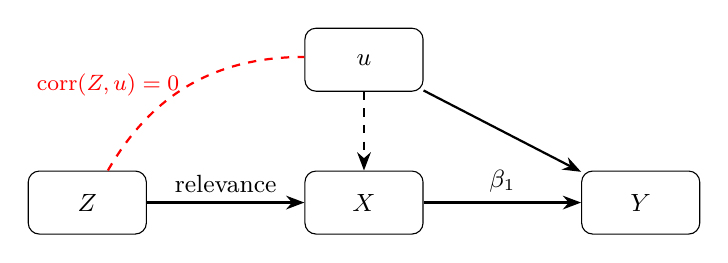
\begin{tikzpicture}[
    >=Stealth,
    box/.style={draw, rounded corners, minimum width=1.5cm, minimum height=0.8cm, align=center},
    every node/.style={font=\small}
  ]
  \node[box] (Z) {$Z$};
  \node[box, right=2cm of Z] (X) {$X$};
  \node[box, right=2cm of X] (Y) {$Y$};
  \node[box, above=1cm of X] (u) {$u$};

  \draw[->, thick] (Z) -- node[above] {relevance} (X);
  \draw[->, thick] (X) -- node[above] {$\beta_1$} (Y);
  \draw[->, thick, dashed] (u) -- (X);
  \draw[->, thick] (u) -- (Y);
  \draw[thick, red, -, dashed] (Z) to[bend left=30] node[left] {\color{red}\footnotesize $\operatorname{corr}(Z,u)=0$} (u);
  % \draw[red, thick] ($(Z)!0.5!(u) + (-0.15,-0.55)$) -- ++(0.3,0.3);
  % \draw[red, thick] ($(Z)!0.5!(u) + (0.15,-0.55)$) -- ++(-0.3,0.3);
\end{tikzpicture}
\end{center}
\end{frame}

\begin{frame}{Two conditions for a valid instrument}
\label{slide:two_conditions}
An instrumental variable $Z$ must satisfy:

\begin{block}{Condition 1: Instrument Relevance}
\[
\operatorname{corr}(Z_i, X_i) \neq 0
\]
$Z$ must be correlated with the endogenous regressor $X$.
\end{block}

\begin{block}{Condition 2: Instrument Exogeneity}
\[
\operatorname{corr}(Z_i, u_i) = 0
\]
$Z$ must be uncorrelated with the error term $u$.
\end{block}

\pause
\begin{alertblock}{Why both are needed}
\begin{itemize}
  \item Relevance without exogeneity $\Rightarrow$ IV captures contaminated variation $\Rightarrow$ inconsistent.
  \item Exogeneity without relevance $\Rightarrow$ $Z$ carries no information about $X$ $\Rightarrow$ division by zero; estimator undefined.
\end{itemize}
\end{alertblock}
\end{frame}

% ============================================================
%  PART 1b: EXOGENEITY -- A DEEPER LOOK
% ============================================================
\section{Exogeneity: A Deeper Look}

\begin{frame}{Three layers of exogeneity}
\label{slide:exogeneity_layers}
Textbooks state instrument exogeneity as $\operatorname{corr}(Z_i,u_i)=0$. But there are three progressively stronger conditions:

\begin{block}{Level 1: Zero Correlation (Weakest)}
\[
\operatorname{cov}(Z_i, u_i) = 0
\]
The \emph{minimum} for TSLS consistency. $Z$ and $u$ are linearly unrelated.
\end{block}

\pause
\begin{block}{Level 2: Mean Independence (Standard)}
\[
E(u_i \mid Z_i) = 0
\]
Knowing $Z$ tells you \alert{nothing} about the average value of $u$. Sufficient for consistency \emph{and} standard asymptotic inference.
\end{block}

\pause
\begin{block}{Level 3: Full Independence (Strongest)}
\[
u_i \perp\!\!\!\perp Z_i
\]
The \emph{entire distribution} of $u$ is unaffected by $Z$. This is what ``as good as randomly assigned'' really means.
\end{block}
\end{frame}

\begin{frame}{Hierarchy: mean independence $\Rightarrow$ zero correlation}
\label{slide:exogeneity_proof}
\begin{block}{Proof: $E(u_i \mid Z_i)=0 \implies \operatorname{cov}(Z_i, u_i)=0$}
By the \emph{law of iterated expectations}:
\begin{align*}
E(Z_i u_i) &= E\bigl[E(Z_i u_i \mid Z_i)\bigr] = E\bigl[Z_i \cdot \underbrace{E(u_i \mid Z_i)}_{=0}\bigr] = 0 \\[4pt]
E(u_i) &= E\bigl[\underbrace{E(u_i \mid Z_i)}_{=0}\bigr] = 0
\end{align*}
Therefore:
\[
\operatorname{cov}(Z_i, u_i) = E(Z_i u_i) - E(Z_i)E(u_i) = 0 - 0 = 0 \qquad \square
\]
\end{block}

\pause
\begin{alertblock}{The converse is FALSE}
$\operatorname{cov}(Z_i, u_i) = 0 \not\!\!\implies E(u_i \mid Z_i) = 0$.

\vspace{0.3em}
\textbf{Counterexample}: Let $Z \sim N(0,1)$ and $u = Z^2 - 1$.
\begin{itemize}
  \item $E(u) = 0$ and $\operatorname{cov}(Z, u) = E(Z^3) - E(Z)E(Z^2-1) = 0$. \checkmark
  \item But $E(u \mid Z=z) = z^2 - 1 \neq 0$ for $z \neq \pm 1$. \ding{55}
\end{itemize}
\end{alertblock}
\end{frame}

\begin{frame}{Why the distinction matters}
\label{slide:exogeneity_why}
\begin{enumerate}
  \item \textbf{Zero correlation} is enough for \alert{consistency} of TSLS.
  \item \textbf{Mean independence} additionally ensures that standard errors, $t$-statistics, and confidence intervals have their usual large-sample properties.
  \item \textbf{Full independence} is the gold standard---implied, for example, when $Z$ is genuinely randomly assigned.
\end{enumerate}

\pause
\vspace{0.5em}
\begin{exampleblock}{Practical implication}
When researchers argue for instrument exogeneity, they typically need arguments strong enough for \emph{at least} mean independence. A variable that satisfies only zero correlation but has nonlinear dependence with $u$ may produce misleading inference even if the point estimate is consistent.
\end{exampleblock}
\end{frame}

\begin{frame}{What happens when exogeneity fails?}
\label{slide:exogeneity_fails}
If $\operatorname{cov}(Z_i, u_i) \neq 0$, the TSLS estimator converges to the \alert{wrong number}:

\[
\hat{\beta}_1^{TSLS} \xrightarrow{p} \beta_1 + \frac{\operatorname{cov}(Z_i, u_i)}{\operatorname{cov}(Z_i, X_i)}
\]

\pause
\begin{itemize}
  \item The \textbf{asymptotic bias} is $\dfrac{\operatorname{cov}(Z_i, u_i)}{\operatorname{cov}(Z_i, X_i)}$.
  \item Compare with OLS bias: $\dfrac{\operatorname{cov}(X_i, u_i)}{\operatorname{var}(X_i)}$.
\end{itemize}

\pause
\begin{alertblock}{Key danger}
Even a \emph{small} violation of exogeneity produces a \emph{large} bias if the instrument is weak ($\operatorname{cov}(Z,X)$ is small). Weak instruments \alert{amplify} exogeneity violations.
\end{alertblock}

\vspace{0.3em}
{\footnotesize\color{gray} See Python notebook: \texttt{lectures/code/01\_exogeneity\_deep\_dive.ipynb} for Monte Carlo simulations.}
\end{frame}

\begin{frame}{How practitioners assess exogeneity}
\label{slide:assess_exogeneity}

\begin{enumerate}
  \item \textbf{Economic reasoning} (always required)
  \begin{itemize}
    \item Argue why $Z$ should affect $Y$ \emph{only through} $X$.
    \item This is the most important step; requires domain expertise.
  \end{itemize}

  \pause
  \item \textbf{Balance / falsification tests}
  \begin{itemize}
    \item Show $Z$ is uncorrelated with \emph{observable} determinants of $Y$.
    \item Regress $Z$ on covariates $W_1, \ldots, W_r$; test joint significance.
    \item If $Z$ is correlated with observables, it is likely correlated with unobservables.
  \end{itemize}

  \pause
  \item \textbf{$J$-test} (when overidentified: $m > k$)
  \begin{itemize}
    \item Tests whether ``extra'' instruments are exogenous.
    \item $J = mF \sim \chi^2_{m-k}$ under $H_0$: all instruments exogenous.
    \item Cannot test the baseline identifying assumption when $m = k$.
  \end{itemize}
\end{enumerate}

\pause
\vspace{0.3em}
\begin{alertblock}{Bottom line}
Exogeneity is ultimately an \alert{assumption}, not something fully verifiable from data. The credibility of IV analysis rests on the persuasiveness of the exogeneity argument.
\end{alertblock}
\end{frame}

% ============================================================
%  PART 1c: THREE SOURCES OF ENDOGENEITY -- IN DETAIL
% ============================================================
\section{Sources of Endogeneity: Theory and Simulation}

\begin{frame}{Roadmap for this section}
\label{slide:endogeneity_roadmap}
We now study each source of endogeneity in detail:
\begin{enumerate}
  \item \textbf{Omitted Variable Bias (OVB)} -- a confounder in the error term
  \item \textbf{Measurement Error (Errors-in-Variables)} -- noise creates a mechanical correlation
  \item \textbf{Simultaneous Causality} -- $X$ and $Y$ are jointly determined
\end{enumerate}

\vspace{0.5em}
For each, we will:
\begin{itemize}
  \item Derive the bias formula mathematically
  \item Show precisely \emph{how} $\operatorname{cov}(X_i, u_i) \neq 0$ arises
  \item Determine the direction and magnitude of the bias
  \item Explain how IV resolves the problem
\end{itemize}

\vspace{0.5em}
{\footnotesize\color{gray} Accompanying simulations: \texttt{lectures/code/02\_sources\_of\_endogeneity.ipynb}}
\end{frame}

% ---------- OVB ----------
\begin{frame}{Source 1: Omitted Variable Bias -- setup}
\label{slide:ovb_setup}
\textbf{True data generating process}:
\[
Y_i = \beta_0 + \beta_1 X_i + \beta_2 W_i + \varepsilon_i, \qquad E(\varepsilon_i \mid X_i, W_i) = 0
\]

\textbf{Estimated model} (we cannot observe $W_i$):
\[
Y_i = \beta_0 + \beta_1 X_i + \underbrace{(\beta_2 W_i + \varepsilon_i)}_{\equiv\; u_i}
\]

\pause
\begin{block}{When does endogeneity arise?}
\[
\operatorname{cov}(X_i, u_i) = \operatorname{cov}(X_i, \beta_2 W_i + \varepsilon_i) = \beta_2 \cdot \operatorname{cov}(X_i, W_i) + \underbrace{\operatorname{cov}(X_i, \varepsilon_i)}_{= 0}
\]
So $\operatorname{cov}(X_i, u_i) \neq 0$ if and only if \alert{both}:
\begin{enumerate}
  \item $\beta_2 \neq 0$: the omitted variable actually affects $Y$
  \item $\operatorname{cov}(X_i, W_i) \neq 0$: the omitted variable is correlated with $X$
\end{enumerate}
\end{block}
\end{frame}

\begin{frame}{Omitted Variable Bias -- the formula}
\label{slide:ovb_formula}
The OLS probability limit when $W$ is omitted:

\[
\hat{\beta}_1^{OLS} \xrightarrow{p} \beta_1 + \underbrace{\beta_2 \cdot \frac{\operatorname{cov}(X_i, W_i)}{\operatorname{var}(X_i)}}_{\text{Omitted Variable Bias}}
\]

\pause
\begin{block}{Direction of bias}
\begin{center}
\begin{tabular}{lcc}
\toprule
& $\operatorname{cov}(X, W) > 0$ & $\operatorname{cov}(X, W) < 0$ \\
\midrule
$\beta_2 > 0$ & \textcolor{red}{Positive bias} $\uparrow$ & \textcolor{blue}{Negative bias} $\downarrow$ \\
$\beta_2 < 0$ & \textcolor{blue}{Negative bias} $\downarrow$ & \textcolor{red}{Positive bias} $\uparrow$ \\
\bottomrule
\end{tabular}
\end{center}
\end{block}

\pause
\begin{exampleblock}{Example}
Estimating the return to education ($X$), omitting ability ($W$). If $\beta_2 > 0$ (ability raises wages) and $\operatorname{cov}(\text{education}, \text{ability}) > 0$ (smarter people get more education), then OLS \alert{overestimates} the return to education.
\end{exampleblock}
\end{frame}

\begin{frame}{OVB -- IV solution}
\label{slide:ovb_iv}
\textbf{Problem}: We cannot include $W$ because it is unobserved.

\textbf{Solution}: Find an instrument $Z$ such that:
\begin{itemize}
  \item $\operatorname{cov}(Z_i, X_i) \neq 0$ \quad (relevance)
  \item $\operatorname{cov}(Z_i, u_i) = \beta_2 \operatorname{cov}(Z_i, W_i) + \operatorname{cov}(Z_i, \varepsilon_i) = 0$ \quad (exogeneity)
\end{itemize}

\pause
The exogeneity condition requires:
\[
\operatorname{cov}(Z_i, W_i) = 0 \quad \text{(and } \operatorname{cov}(Z_i, \varepsilon_i) = 0\text{)}
\]
The instrument must be \alert{uncorrelated with the omitted variable}.

\pause
\vspace{0.5em}
\begin{exampleblock}{Example (Angrist \& Krueger, 1991)}
Return to education ($X$), omitting ability ($W$).\\
Instrument: \emph{quarter of birth} ($Z$) -- affects years of schooling through compulsory schooling laws, but is plausibly unrelated to innate ability.
\end{exampleblock}
\end{frame}

% ---------- MEASUREMENT ERROR ----------
\begin{frame}{Source 2: Measurement Error -- setup}
\label{slide:meas_err_setup}
\textbf{True model}: $Y_i = \beta_0 + \beta_1 X_i^* + \varepsilon_i, \quad E(\varepsilon_i \mid X_i^*) = 0$

where $X_i^*$ is the \emph{true} value (unobserved). We observe:
\[
X_i = X_i^* + w_i
\]
with \textbf{classical measurement error}: $E(w_i) = 0$, $\operatorname{cov}(w_i, X_i^*) = 0$, $\operatorname{cov}(w_i, \varepsilon_i) = 0$.

\pause
Substitute $X_i^* = X_i - w_i$ into the true model:
\[
Y_i = \beta_0 + \beta_1 X_i + \underbrace{(\varepsilon_i - \beta_1 w_i)}_{\equiv\; u_i}
\]

\pause
\begin{alertblock}{The endogeneity}
\vspace{-0.5em}
\begin{align*}
\operatorname{cov}(X_i, u_i) &= \operatorname{cov}(X_i^* + w_i, \; \varepsilon_i - \beta_1 w_i)\\
&= \underbrace{\operatorname{cov}(X_i^*, \varepsilon_i)}_{0} - \beta_1\underbrace{\operatorname{cov}(X_i^*, w_i)}_{0}
 + \underbrace{\operatorname{cov}(w_i, \varepsilon_i)}_{0} - \beta_1 \underbrace{\operatorname{var}(w_i)}_{\sigma_w^2} \\
&= -\beta_1 \sigma_w^2 \neq 0
\end{align*}
\end{alertblock}
\end{frame}

\begin{frame}{Measurement Error -- attenuation bias}
\label{slide:attenuation}
The OLS probability limit:
\begin{align*}
\hat{\beta}_1^{OLS} &\xrightarrow{p} \beta_1 + \frac{\operatorname{cov}(X_i, u_i)}{\operatorname{var}(X_i)} = \beta_1 + \frac{-\beta_1 \sigma_w^2}{\sigma_{X^*}^2 + \sigma_w^2} \\[6pt]
&= \beta_1 \left(\frac{\sigma_{X^*}^2}{\sigma_{X^*}^2 + \sigma_w^2}\right)
\end{align*}

\pause
Since $\dfrac{\sigma_{X^*}^2}{\sigma_{X^*}^2 + \sigma_w^2} < 1$:

\begin{block}{Attenuation bias}
OLS with classical measurement error is \alert{biased toward zero}. The coefficient is ``attenuated.''
\begin{itemize}
  \item If $\beta_1 > 0$: OLS underestimates the true effect.
  \item If $\beta_1 < 0$: OLS overestimates (closer to zero) the true effect.
  \item More noise ($\sigma_w^2 \uparrow$) $\Rightarrow$ more attenuation.
\end{itemize}
\end{block}

\pause
\vspace{0.3em}
{\small The ratio $\lambda = \sigma_{X^*}^2 / (\sigma_{X^*}^2 + \sigma_w^2)$ is called the \textbf{reliability ratio} or \textbf{signal-to-total-variance ratio}.}
\end{frame}

\begin{frame}{Measurement Error -- IV solution}
\label{slide:meas_err_iv}
We need an instrument $Z$ such that:
\begin{itemize}
  \item $\operatorname{cov}(Z_i, X_i) \neq 0$ \quad (relevance -- $Z$ predicts the \emph{noisy} $X$)
  \item $\operatorname{cov}(Z_i, u_i) = \operatorname{cov}(Z_i, \varepsilon_i) - \beta_1 \operatorname{cov}(Z_i, w_i) = 0$ \quad (exogeneity)
\end{itemize}

\pause
The exogeneity condition requires:
\[
\operatorname{cov}(Z_i, w_i) = 0 \quad \text{and} \quad \operatorname{cov}(Z_i, \varepsilon_i) = 0
\]
The instrument must be uncorrelated with the \alert{measurement noise}.

\pause
\vspace{0.5em}
\begin{exampleblock}{What instruments work?}
\begin{itemize}
  \item A \emph{second independent measurement} of $X^*$ (e.g., a different survey question measuring the same concept)
  \item Any variable that predicts $X^*$ but is unrelated to the measurement noise $w$ and the structural error $\varepsilon$
\end{itemize}
\end{exampleblock}
\end{frame}

% ---------- SIMULTANEOUS CAUSALITY ----------
\begin{frame}{Source 3: Simultaneous Causality -- setup}
\label{slide:simul_setup}
\textbf{System of simultaneous equations} (supply and demand):
\begin{align*}
\text{Demand}: \quad Q_i &= \alpha_0 + \alpha_1 P_i + u_i^d \qquad (\alpha_1 < 0) \\
\text{Supply}: \quad Q_i &= \gamma_0 + \gamma_1 P_i + u_i^s \qquad (\gamma_1 > 0)
\end{align*}

\textbf{Equilibrium}: $Q_i^d = Q_i^s$ simultaneously determines both $P_i$ and $Q_i$.

\pause
\vspace{0.5em}
Setting demand $=$ supply and solving for the equilibrium price:
\[
P_i = \frac{(\gamma_0 - \alpha_0) + (u_i^s - u_i^d)}{\alpha_1 - \gamma_1}
\]

\pause
\begin{alertblock}{Key observation}
The equilibrium price $P_i$ depends on the demand shock $u_i^d$. So $\operatorname{cov}(P_i, u_i^d) \neq 0$: the regressor in the demand equation is \alert{endogenous}.
\end{alertblock}
\end{frame}

\begin{frame}{Simultaneous Causality -- deriving the bias}
\label{slide:simul_bias}
\textbf{Goal}: Estimate the demand elasticity $\alpha_1$ from $Q_i = \alpha_0 + \alpha_1 P_i + u_i^d$.

\pause
Compute the covariance (assuming $u^d \perp u^s$, both mean-zero):
\[
\operatorname{cov}(P_i, u_i^d) = \operatorname{cov}\!\left(\frac{u_i^s - u_i^d}{\alpha_1 - \gamma_1},\; u_i^d\right) = \frac{-\sigma_d^2}{\alpha_1 - \gamma_1}
\]
Since $\alpha_1 - \gamma_1 < 0$, we get $\operatorname{cov}(P_i, u_i^d) > 0$.

\pause
\vspace{0.5em}
\begin{block}{OLS probability limit}
\[
\hat{\alpha}_1^{OLS} \xrightarrow{p} \frac{\alpha_1 \sigma_s^2 + \gamma_1 \sigma_d^2}{\sigma_s^2 + \sigma_d^2}
\]
This is a \alert{variance-weighted average} of the demand slope $\alpha_1$ and the supply slope $\gamma_1$. OLS estimates \emph{neither} curve---it gives a meaningless hybrid.
\end{block}
\end{frame}

\begin{frame}{Wright's insight: shifting one curve to identify the other}
\label{slide:wright_insight}
\begin{center}
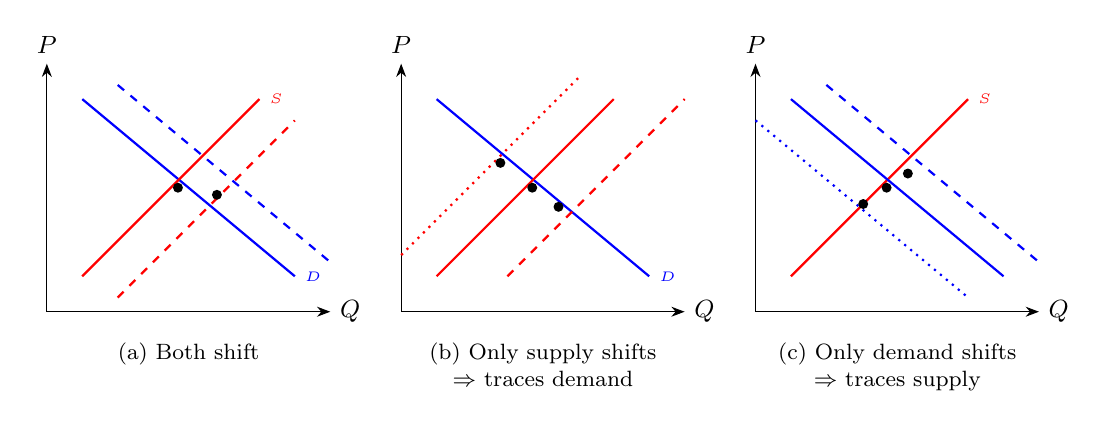
\begin{tikzpicture}[>=Stealth, scale=0.9]
  % Panel (a): Both shift
  \begin{scope}[shift={(-5,0)}]
    \draw[->] (0,0) -- (4,0) node[right] {\small $Q$};
    \draw[->] (0,0) -- (0,3.5) node[above] {\small $P$};
    \draw[blue, thick] (0.5,3) -- (3.5,0.5) node[right] {\tiny $D$};
    \draw[red, thick] (0.5,0.5) -- (3,3) node[right] {\tiny $S$};
    \fill (1.85,1.75) circle (2pt);
    \draw[blue, thick, dashed] (1,3.2) -- (4,0.7);
    \draw[red, thick, dashed] (1,0.2) -- (3.5,2.7);
    \fill (2.4,1.65) circle (2pt);
    \node[below] at (2,-0.3) {\footnotesize (a) Both shift};
  \end{scope}
  % Panel (b): Only S shifts
  \begin{scope}[shift={(0,0)}]
    \draw[->] (0,0) -- (4,0) node[right] {\small $Q$};
    \draw[->] (0,0) -- (0,3.5) node[above] {\small $P$};
    \draw[blue, thick] (0.5,3) -- (3.5,0.5) node[right] {\tiny $D$};
    \draw[red, thick] (0.5,0.5) -- (3,3);
    \draw[red, thick, dashed] (1.5,0.5) -- (4,3);
    \draw[red, thick, dotted] (0,0.8) -- (2.5,3.3);
    \fill (1.85,1.75) circle (2pt);
    \fill (2.22,1.48) circle (2pt);
    \fill (1.4,2.1) circle (2pt);
    \node[below] at (2,-0.3) {\footnotesize (b) Only supply shifts};
    \node[below] at (2,-0.7) {\footnotesize $\Rightarrow$ traces demand};
  \end{scope}
  % Panel (c): Only D shifts
  \begin{scope}[shift={(5,0)}]
    \draw[->] (0,0) -- (4,0) node[right] {\small $Q$};
    \draw[->] (0,0) -- (0,3.5) node[above] {\small $P$};
    \draw[red, thick] (0.5,0.5) -- (3,3) node[right] {\tiny $S$};
    \draw[blue, thick] (0.5,3) -- (3.5,0.5);
    \draw[blue, thick, dashed] (1,3.2) -- (4,0.7);
    \draw[blue, thick, dotted] (0,2.7) -- (3,0.2);
    \fill (1.85,1.75) circle (2pt);
    \fill (2.15,1.95) circle (2pt);
    \fill (1.52,1.52) circle (2pt);
    \node[below] at (2,-0.3) {\footnotesize (c) Only demand shifts};
    \node[below] at (2,-0.7) {\footnotesize $\Rightarrow$ traces supply};
  \end{scope}
\end{tikzpicture}
\end{center}

\vspace{0.5em}
\textbf{IV idea}: Find a variable $Z$ that shifts \emph{only supply} (a \alert{supply shifter}). Then variation in equilibrium $(P, Q)$ traces out the demand curve $\Rightarrow$ we can estimate $\alpha_1$.
\end{frame}

\begin{frame}{Simultaneous Causality -- IV solution}
\label{slide:simul_iv}
To estimate the \textbf{demand} elasticity, we need a \alert{supply shifter} $Z$:
\begin{itemize}
  \item Include $Z$ in the supply equation: $Q_i = \gamma_0 + \gamma_1 P_i + \delta Z_i + u_i^s$
  \item $Z$ is relevant: $\operatorname{cov}(Z_i, P_i) \neq 0$ (shifting supply changes equilibrium price)
  \item $Z$ is exogenous: $\operatorname{cov}(Z_i, u_i^d) = 0$ ($Z$ does not directly shift demand)
\end{itemize}

\pause
\vspace{0.5em}
\begin{exampleblock}{Examples of supply shifters for demand estimation}
\begin{itemize}
  \item Philip Wright: \emph{rainfall} in dairy regions $\to$ butter supply
  \item Cigarette taxes: \emph{excise taxes} shift supply (increase after-tax price)
  \item Oil market: \emph{geopolitical disruptions} shift oil supply
\end{itemize}
\end{exampleblock}

\pause
\vspace{0.3em}
To estimate the \textbf{supply} elasticity, reverse the logic: use a \alert{demand shifter} as the instrument (e.g., income shocks, population changes).
\end{frame}

\begin{frame}{Summary: three sources, one unified framework}
\label{slide:sources_summary}

\begin{center}
\small
\begin{tabular}{p{2.5cm}p{3cm}p{2.5cm}p{2.7cm}}
\toprule
\textbf{Source} & \textbf{Why $\operatorname{cov}(X,u) \neq 0$} & \textbf{OLS bias direction} & \textbf{IV requirement} \\
\midrule
Omitted variables & $u$ contains $W$; $W$ correlated with $X$ & Depends on signs of $\beta_2$, $\operatorname{cov}(X,W)$ & $Z$ uncorrelated with $W$ \\[6pt]
Measurement error & $w$ enters both $X$ and $u$ & \alert{Toward zero} (attenuation) & $Z$ uncorrelated with $w$ \\[6pt]
Simultaneity & $X$ determined by equilibrium involving $u$ & Toward ``other equation'' slope & $Z$ shifts other equation only \\
\bottomrule
\end{tabular}
\end{center}

\pause
\vspace{0.5em}
\begin{block}{The common thread}
All three create $\operatorname{cov}(X_i, u_i) \neq 0$. IV provides a \alert{unified solution}: find a variable $Z$ that isolates exogenous variation in $X$.
\end{block}

\vspace{0.3em}
{\footnotesize\color{gray} Full Monte Carlo simulations: \texttt{lectures/code/02\_sources\_of\_endogeneity.ipynb}}
\end{frame}

% ============================================================
%  PART 2: TSLS ESTIMATOR -- SIMPLE CASE
% ============================================================
\section{The Two Stage Least Squares (TSLS) Estimator}

\begin{frame}{TSLS: the big picture}
\label{slide:tsls_overview}
\textbf{Goal}: Isolate the exogenous variation in $X$ and use only that to estimate $\beta_1$.

\vspace{0.5em}
\textbf{Two stages}:
\begin{enumerate}
  \item \textbf{First stage}: Regress $X$ on $Z$ to extract the ``clean'' component.
  \item \textbf{Second stage}: Regress $Y$ on the predicted $\hat{X}$ from stage 1.
\end{enumerate}

\pause
\vspace{0.5em}
\begin{exampleblock}{Intuition}
The first stage \emph{purifies} $X$ by projecting it onto the instrument $Z$. The predicted value $\hat{X}$ inherits $Z$'s exogeneity.  The second stage uses only this purified variation.
\end{exampleblock}
\end{frame}

\begin{frame}{First stage: decomposing $X$}
\label{slide:first_stage}
The population first-stage regression:
\begin{equation}
X_i = \pi_0 + \pi_1 Z_i + v_i \tag{12.2}
\end{equation}

\begin{itemize}
  \item $\pi_0 + \pi_1 Z_i$: the part of $X_i$ that can be predicted by $Z_i$.\\
        Because $Z_i$ is exogenous, this component is \alert{uncorrelated with $u_i$}.
  \item $v_i$: the ``remainder'' -- this is the \alert{problematic} part correlated with $u_i$.
\end{itemize}

\pause
\vspace{0.5em}
In practice, $\pi_0$ and $\pi_1$ are unknown. We estimate them by OLS:
\[
\hat{X}_i = \hat{\pi}_0 + \hat{\pi}_1 Z_i
\]

$\hat{X}_i$ is the \textbf{fitted value} from the first stage.
\end{frame}

\begin{frame}{Second stage: using the purified $\hat{X}$}
\label{slide:second_stage}
\textbf{Second stage}: Regress $Y_i$ on $\hat{X}_i$ using OLS.

\[
Y_i = \beta_0 + \beta_1 \hat{X}_i + \text{error}_i
\]

The OLS estimators from this second-stage regression are the TSLS estimators $\hat{\beta}_0^{TSLS}$ and $\hat{\beta}_1^{TSLS}$.

\pause
\vspace{1em}
\begin{alertblock}{Important practical note}
In practice, both stages are performed automatically by econometric software. The standard errors from a ``manual'' second-stage OLS regression are \alert{incorrect} because they do not account for the estimation uncertainty from the first stage.
\end{alertblock}
\end{frame}

\begin{frame}{The TSLS formula: $\hat{\beta}_1^{TSLS} = s_{ZY}/s_{ZX}$}
\label{slide:tsls_formula}
\begin{block}{Theorem (TSLS Formula)}
With a single regressor $X$ and a single instrument $Z$:
\[
\hat{\beta}_1^{TSLS} = \frac{s_{ZY}}{s_{ZX}}
\]
where $s_{ZY}$ is the sample covariance between $Z$ and $Y$, and $s_{ZX}$ is the sample covariance between $Z$ and $X$.
\end{block}

\pause
\textbf{Interpretation}: The TSLS estimator is the ratio of the reduced-form effect ($Z \to Y$) to the first-stage effect ($Z \to X$). This is sometimes called the \alert{Wald estimator}.
\end{frame}

\begin{frame}{Deriving the TSLS formula (Appendix 12.2)}
\label{slide:tsls_derivation}
The TSLS estimator is, by definition, the OLS slope from regressing $Y$ on $\hat{X}$:
\[
\hat{\beta}_1^{TSLS} = \frac{s_{\hat{X}Y}}{s_{\hat{X}}^2}
\]

\pause
Since $\hat{X}_i = \hat{\pi}_0 + \hat{\pi}_1 Z_i$, we can compute:
\begin{align*}
s_{\hat{X}Y} &= \hat{\pi}_1 \, s_{ZY} \\[4pt]
s_{\hat{X}}^2 &= \hat{\pi}_1^2 \, s_Z^2
\end{align*}

\pause
Therefore:
\[
\hat{\beta}_1^{TSLS} = \frac{\hat{\pi}_1 \, s_{ZY}}{\hat{\pi}_1^2 \, s_Z^2} = \frac{s_{ZY}}{\hat{\pi}_1 \, s_Z^2}
\]

\pause
But $\hat{\pi}_1 = s_{ZX}/s_Z^2$ (the OLS slope from the first stage), so:
\[
\hat{\beta}_1^{TSLS} = \frac{s_{ZY}}{(s_{ZX}/s_Z^2) \cdot s_Z^2} = \boxed{\frac{s_{ZY}}{s_{ZX}}} \qed
\]
\end{frame}

% ============================================================
%  PART 3: WHY IV WORKS -- CONSISTENCY
% ============================================================
\section{Why IV Works: Consistency of TSLS}

\begin{frame}{Consistency of TSLS: the key insight}
\label{slide:consistency}
Starting from $Y_i = \beta_0 + \beta_1 X_i + u_i$, take covariances with $Z_i$:

\pause
\begin{align}
\operatorname{cov}(Z_i, Y_i) &= \operatorname{cov}(Z_i, \beta_0 + \beta_1 X_i + u_i) \notag \\[4pt]
&= \beta_1 \operatorname{cov}(Z_i, X_i) + \operatorname{cov}(Z_i, u_i) \tag{12.5}
\end{align}

\pause
Under \alert{instrument exogeneity}: $\operatorname{cov}(Z_i, u_i) = 0$.

Under \alert{instrument relevance}: $\operatorname{cov}(Z_i, X_i) \neq 0$.

\pause
Solving:
\[
\boxed{\beta_1 = \frac{\operatorname{cov}(Z_i, Y_i)}{\operatorname{cov}(Z_i, X_i)}} \tag{12.6}
\]

This is the \textbf{population} analog of the TSLS formula.
\end{frame}

\begin{frame}{From population to sample: consistency}
\label{slide:consistency_proof}
The sample covariance is a consistent estimator of the population covariance:
\[
s_{ZY} \xrightarrow{p} \operatorname{cov}(Z_i, Y_i), \qquad s_{ZX} \xrightarrow{p} \operatorname{cov}(Z_i, X_i)
\]

\pause
Therefore, by the continuous mapping theorem (Slutsky):
\[
\hat{\beta}_1^{TSLS} = \frac{s_{ZY}}{s_{ZX}} \xrightarrow{p} \frac{\operatorname{cov}(Z_i, Y_i)}{\operatorname{cov}(Z_i, X_i)} = \beta_1 \tag{12.7}
\]

\pause
\begin{exampleblock}{Key takeaway}
The TSLS estimator is \textbf{consistent} for $\beta_1$ under the two conditions for instrument validity. This holds regardless of the correlation between $X$ and $u$ -- the endogeneity that plagues OLS is completely circumvented.
\end{exampleblock}
\end{frame}

% ============================================================
%  PART 4: SAMPLING DISTRIBUTION
% ============================================================
\section{Sampling Distribution of the TSLS Estimator}

\begin{frame}{Expressing TSLS in terms of errors}
\label{slide:tsls_errors}
From $Y_i - \bar{Y} = \beta_1(X_i - \bar{X}) + (u_i - \bar{u})$, substitute into $s_{ZY}$:
\begin{align*}
s_{ZY} &= \frac{1}{n-1}\sum_{i=1}^n (Z_i - \bar{Z})(Y_i - \bar{Y}) \\
       &= \beta_1 s_{ZX} + \frac{1}{n-1}\sum_{i=1}^n (Z_i - \bar{Z})u_i
\end{align*}

\pause
where the last step uses $\sum(Z_i - \bar{Z})\bar{u} = 0$.

Dividing by $s_{ZX}$ and multiplying numerator and denominator by $(n{-}1)/n$:
\[
\boxed{\hat{\beta}_1^{TSLS} = \beta_1 + \frac{\frac{1}{n}\sum_{i=1}^n (Z_i - \bar{Z})u_i}{\frac{1}{n}\sum_{i=1}^n (Z_i - \bar{Z})(X_i - \bar{X})}} \tag{12.20}
\]

This is the fundamental equation for analyzing the distribution of TSLS.
\end{frame}

\begin{frame}{Asymptotic normality of TSLS (Appendix 12.3)}
\label{slide:asymptotic_normality}
From Eq.\ (12.20), focus on the \alert{numerator}:
\[
\bar{q} = \frac{1}{n}\sum_{i=1}^n (Z_i - \bar{Z})u_i \approx \frac{1}{n}\sum_{i=1}^n \underbrace{(Z_i - \mu_Z)u_i}_{q_i}
\]

\pause
\begin{itemize}
  \item $E(q_i) = 0$ \quad (by instrument exogeneity).
  \item $q_i$ is i.i.d.\ with variance $\sigma_q^2 = \operatorname{var}[(Z_i - \mu_Z)u_i]$.
  \item By the \alert{CLT}: $\dfrac{\sqrt{n}\,\bar{q}}{\sigma_q} \xrightarrow{d} N(0,1)$.
\end{itemize}

\pause
The \alert{denominator} converges in probability:
\[
\frac{1}{n}\sum_{i=1}^n (Z_i - \bar{Z})(X_i - \bar{X}) \xrightarrow{p} \operatorname{cov}(Z_i, X_i) \neq 0
\]

By \textbf{Slutsky's theorem}, the ratio is asymptotically normal.
\end{frame}

\begin{frame}{The large-sample distribution of TSLS}
\label{slide:large_sample}

\begin{block}{Theorem (Large-Sample Distribution)}
Under the IV regression assumptions:
\[
\hat{\beta}_1^{TSLS} \stackrel{a}{\sim} N\!\left(\beta_1, \;\sigma_{\hat{\beta}_1^{TSLS}}^2\right)
\]
where
\[
\sigma_{\hat{\beta}_1^{TSLS}}^2 = \frac{1}{n}\cdot\frac{\operatorname{var}\!\big[(Z_i - \mu_Z)u_i\big]}{\big[\operatorname{cov}(Z_i, X_i)\big]^2} \tag{12.8}
\]
\end{block}

\pause
\textbf{Key observations}:
\begin{itemize}
  \item Variance decreases at rate $1/n$ (as expected).
  \item Variance is \alert{larger} when $\operatorname{cov}(Z_i,X_i)$ is small $\Rightarrow$ weak instruments inflate variance.
  \item When $Z = X$ and $\operatorname{cov}(Z,u)=0$: reduces to OLS variance.
\end{itemize}
\end{frame}

\begin{frame}{Statistical inference with TSLS}
\label{slide:inference}
Because $\hat{\beta}_1^{TSLS}$ is asymptotically normal:

\begin{itemize}
  \item \textbf{$t$-statistic}: $t = \dfrac{\hat{\beta}_1^{TSLS} - \beta_{1,0}}{SE(\hat{\beta}_1^{TSLS})}$

  \medskip
  \item \textbf{95\% confidence interval}: $\hat{\beta}_1^{TSLS} \pm 1.96 \cdot SE(\hat{\beta}_1^{TSLS})$
\end{itemize}

\pause
\vspace{0.5em}
\begin{alertblock}{Two practical warnings}
\begin{enumerate}
  \item \textbf{Use TSLS standard errors}, not manual second-stage OLS standard errors (the latter are incorrect because they ignore first-stage estimation uncertainty).
  \item \textbf{Use heteroskedasticity-robust standard errors} -- exactly as with OLS.
\end{enumerate}
\end{alertblock}
\end{frame}

% ============================================================
%  PART 5: ILLUSTRATIVE EXAMPLES
% ============================================================
\section{Illustrative Examples}

\begin{frame}{Philip Wright's problem: supply and demand for butter}
\label{slide:wright}
Philip Wright (1928) wanted to estimate the \alert{demand elasticity for butter}:
\[
\ln(Q_i^{butter}) = \beta_0 + \beta_1 \ln(P_i^{butter}) + u_i
\]

\pause
\textbf{The problem}:
\begin{itemize}
  \item Price and quantity are \emph{jointly} determined by supply and demand.
  \item Both curves shift over time $\Rightarrow$ equilibrium points trace out \emph{neither} curve.
  \item OLS on the scatter of $(P,Q)$ points estimates a meaningless hybrid.
\end{itemize}

\pause
\textbf{Wright's insight}: Find a variable that shifts \emph{supply only} (not demand).
\begin{itemize}
  \item When only supply shifts, the equilibrium traces out the \alert{demand curve}.
  \item Instrument: \textbf{dairy-region rainfall}.
\end{itemize}
\end{frame}

\begin{frame}{Why rainfall works as an instrument}
\label{slide:rainfall_instrument}

\begin{columns}[T,onlytextwidth]
\column{0.55\textwidth}
\textbf{Relevance}: Below-average rainfall impairs grazing $\Rightarrow$ reduces butter supply $\Rightarrow$ raises equilibrium price.
\[
\operatorname{corr}(\text{Rainfall}, \ln P^{butter}) \neq 0 \;\checkmark
\]

\vspace{0.5em}
\textbf{Exogeneity}: Dairy-region rainfall has no direct effect on consumer \emph{demand} for butter.
\[
\operatorname{corr}(\text{Rainfall}, u_i) = 0 \;\checkmark
\]

\column{0.42\textwidth}
\begin{block}{Supply--demand diagram intuition}
\small
\begin{itemize}
  \item Both curves shift: scatter of equilibria $\Rightarrow$ can't identify either curve.
  \item Only supply shifts: equilibria lie on the stable demand curve $\Rightarrow$ slope = demand elasticity.
\end{itemize}
\end{block}
\end{columns}

\pause
\vspace{0.5em}
\begin{exampleblock}{Historical note}
IV regression was invented by Philip G.\ Wright and his son Sewall Wright (a geneticist) in \emph{The Tariff on Animal and Vegetable Oils} (1928). The intellectual approach was anticipated by John Snow's 1855 cholera study, which used water company source as an instrument for exposure to contaminated water.
\end{exampleblock}
\end{frame}

\begin{frame}{Application: demand elasticity for cigarettes}
\label{slide:cigarettes_intro}
\textbf{Policy question}: How much must cigarette taxes rise to reduce consumption by 20\%?

\vspace{0.3em}
Answer depends on the \alert{price elasticity of demand}:
\[
\ln(Q_i^{cig}) = \beta_0 + \beta_1 \ln(P_i^{cig}) + u_i
\]

\pause
\begin{itemize}
  \item OLS is inconsistent: simultaneous causality between price and quantity.
  \item \textbf{Instrument}: $\text{SalesTax}_i$ (general state sales tax per pack).
\end{itemize}

\pause
\textbf{First stage} (48 U.S.\ states, 1995):
\[
\widehat{\ln(P_i^{cig})} = \underset{(0.03)}{4.62} + \underset{(0.005)}{0.031}\;\text{SalesTax}_i, \qquad R^2 = 0.47
\]

\textbf{TSLS (second stage)}:
\[
\widehat{\ln(Q_i^{cig})} = \underset{(1.53)}{9.72} - \underset{(0.32)}{1.08}\;\ln(P_i^{cig})
\]

Demand is elastic: a 1\% price increase reduces consumption by 1.08\%.
\end{frame}

% ============================================================
%  PART 6: THE GENERAL IV REGRESSION MODEL
% ============================================================
\section{The General IV Regression Model}

\begin{frame}{The general model (Key Concept 12.1)}
\label{slide:general_model}
\begin{block}{General IV Regression Model}
\vspace{-0.5em}
\begin{equation}
Y_i = \beta_0 + \underbrace{\beta_1 X_{1i} + \cdots + \beta_k X_{ki}}_{\text{endogenous regressors}} + \underbrace{\beta_{k+1}W_{1i} + \cdots + \beta_{k+r}W_{ri}}_{\text{included exogenous/control variables}} + u_i \tag{12.12}
\end{equation}
\end{block}

\textbf{Four types of variables}:
\begin{enumerate}
  \item $Y_i$: dependent variable
  \item $X_{1i}, \ldots, X_{ki}$: $k$ \alert{endogenous} regressors (correlated with $u_i$)
  \item $W_{1i}, \ldots, W_{ri}$: $r$ \alert{exogenous} regressors or control variables
  \item $Z_{1i}, \ldots, Z_{mi}$: $m$ \alert{instrumental variables} (excluded from the structural equation)
\end{enumerate}
\end{frame}

\begin{frame}{Identification: counting instruments vs.\ endogenous regressors}
\label{slide:identification}
The relationship between the number of instruments ($m$) and endogenous regressors ($k$) determines identification:

\begin{center}
\renewcommand{\arraystretch}{1.3}
\begin{tabular}{@{}lll@{}}
\toprule
\textbf{Case} & \textbf{Condition} & \textbf{Implication} \\
\midrule
Exactly identified & $m = k$ & Can estimate; unique TSLS solution \\
Overidentified & $m > k$ & Can estimate; can test overidentifying restrictions \\
\alert{Underidentified} & $m < k$ & \alert{Cannot estimate}; not enough instruments \\
\bottomrule
\end{tabular}
\end{center}

\pause
\begin{exampleblock}{Order condition (necessary)}
IV regression requires \alert{at least as many instruments as endogenous regressors}: $m \geq k$.
\end{exampleblock}
\end{frame}

\begin{frame}{TSLS in the general model (Key Concept 12.2)}
\label{slide:tsls_general}
\begin{block}{Two Stage Least Squares -- General Case}
\textbf{First stage}: For each endogenous regressor $X_{ji}$ ($j=1,\ldots,k$), run the OLS regression:
\[
X_{ji} = \pi_0 + \pi_1 Z_{1i} + \cdots + \pi_m Z_{mi} + \pi_{m+1}W_{1i} + \cdots + \pi_{m+r}W_{ri} + v_{ji}
\]
Obtain predicted values $\hat{X}_{1i}, \ldots, \hat{X}_{ki}$.

\vspace{0.5em}
\textbf{Second stage}: Regress $Y_i$ on $\hat{X}_{1i}, \ldots, \hat{X}_{ki}, W_{1i}, \ldots, W_{ri}$ using OLS.

\vspace{0.5em}
The resulting estimators are $\hat{\beta}_0^{TSLS}, \hat{\beta}_1^{TSLS}, \ldots, \hat{\beta}_{k+r}^{TSLS}$.
\end{block}

\pause
\vspace{0.3em}
\textbf{Key points}:
\begin{itemize}
  \item Each first-stage regression includes \alert{all} instruments and \alert{all} exogenous regressors.
  \item In practice, both stages are computed automatically by TSLS commands.
\end{itemize}
\end{frame}

\begin{frame}{General conditions for valid instruments (Key Concept 12.3)}
\label{slide:general_validity}
A set of instruments $Z_{1i}, \ldots, Z_{mi}$ is valid if:

\begin{block}{1. Instrument Relevance}
Let $\hat{X}_{ji}^*$ be the predicted value from the \emph{population} regression of $X_{ji}$ on all $Z$'s and $W$'s. Then $(\hat{X}_{1i}^*, \ldots, \hat{X}_{ki}^*, W_{1i}, \ldots, W_{ri}, 1)$ are \textbf{not perfectly multicollinear}.

\vspace{0.3em}
\emph{When $k=1$}: at least one $Z$ has a nonzero coefficient in the population regression of $X$ on the $Z$'s and $W$'s.
\end{block}

\begin{block}{2. Instrument Exogeneity}
\[
\operatorname{corr}(Z_{1i}, u_i) = 0, \quad \ldots, \quad \operatorname{corr}(Z_{mi}, u_i) = 0
\]
\emph{All} instruments must be uncorrelated with the error term.
\end{block}
\end{frame}

\begin{frame}{IV regression assumptions (Key Concept 12.4)}
\label{slide:iv_assumptions}
\begin{block}{The Four IV Regression Assumptions}
\begin{enumerate}
  \item $E(u_i \mid W_{1i}, \ldots, W_{ri}) = 0$.\\
  {\small (Exogenous variables/controls are uncorrelated with $u$ in the conditional mean sense.)}

  \item $(X_{1i}, \ldots, X_{ki}, W_{1i}, \ldots, W_{ri}, Z_{1i}, \ldots, Z_{mi}, Y_i)$ are \textbf{i.i.d.} draws.\\
  {\small (Satisfied under simple random sampling.)}

  \item \textbf{Large outliers are unlikely}: all $X$'s, $W$'s, $Z$'s, and $Y$ have nonzero finite fourth moments.

  \item The two conditions for \textbf{valid instruments} (relevance + exogeneity) hold.
\end{enumerate}
\end{block}

\pause
Under these assumptions, $\hat{\beta}^{TSLS}$ is \alert{consistent} and \alert{asymptotically normal}.
\end{frame}

\begin{frame}{The role of control variables ($W$'s) in IV regression}
\label{slide:controls}
Why include exogenous variables $W$ in the IV regression?

\begin{enumerate}
  \item \textbf{Making instruments exogenous}: If $Z$ is correlated with an omitted variable, but that variable is observable, include it as $W$. This breaks the correlation between $Z$ and $u$.

  \pause
  \item \textbf{Improving precision}: Even if $Z$ is already exogenous, including relevant $W$'s reduces residual variance $\Rightarrow$ smaller standard errors.
\end{enumerate}

\pause
\begin{exampleblock}{Cigarette demand example}
Sales tax might correlate with state income, which affects demand. Including $\ln(\text{Inc}_i)$ as $W$ breaks this correlation, making SalesTax a more credibly exogenous instrument:
\[
\widehat{\ln(Q_i^{cig})} = \underset{(1.26)}{9.43} - \underset{(0.37)}{1.14}\;\ln(P_i^{cig}) + \underset{(0.31)}{0.21}\;\ln(\text{Inc}_i)
\]
\end{exampleblock}
\end{frame}

% ============================================================
%  PART 7: CHECKING INSTRUMENT VALIDITY
% ============================================================
\section{Checking Instrument Validity}

\begin{frame}{Weak instruments: why they are dangerous}
\label{slide:weak_intro}
If instruments explain very little of the variation in $X$, they are called \alert{weak instruments}.

\vspace{0.5em}
\textbf{Consequences of weak instruments}:
\begin{enumerate}
  \item TSLS is \alert{biased toward OLS}, even in large samples.
  \item The normal approximation to the sampling distribution is \alert{poor} $\Rightarrow$ $t$-statistics and confidence intervals are unreliable.
  \item 95\% CIs may contain the true value far less than 95\% of the time.
\end{enumerate}

\pause
\begin{alertblock}{Extreme case: irrelevant instrument}
When $\operatorname{cov}(Z_i, X_i) = 0$, the denominator $s_{ZX} \xrightarrow{p} 0$. The large-sample distribution of TSLS becomes the \textbf{ratio of two normal random variables} (not normal!), centered on the probability limit of OLS.
\end{alertblock}
\end{frame}

\begin{frame}{Weak instruments: the formal argument}
\label{slide:weak_formal}
From Eq.\ (12.20): $\hat{\beta}_1^{TSLS} = \beta_1 + \bar{q}/\bar{r}$ where:
\begin{align*}
\bar{q} &= \frac{1}{n}\sum (Z_i - \bar{Z})u_i \xrightarrow{d} N(0, \sigma_q^2/n) \\
\bar{r} &= \frac{1}{n}\sum (Z_i - \bar{Z})(X_i - \bar{X})
\end{align*}

\pause
\textbf{When instrument is relevant}: $E(\bar{r}) = \operatorname{cov}(Z,X) \neq 0$ $\Rightarrow$ $\bar{r} \xrightarrow{p} \operatorname{cov}(Z,X)$ $\Rightarrow$ Slutsky applies $\Rightarrow$ normal distribution.

\pause
\textbf{When instrument is irrelevant}: $E(\bar{r}) = 0$ $\Rightarrow$ CLT applies to \emph{both} numerator and denominator:
\[
\hat{\beta}_1^{TSLS} - \beta_1 \approx \frac{\sigma_q}{\sigma_r}\cdot\frac{\bar{q}/\sigma_{\bar{q}}}{\bar{r}/\sigma_{\bar{r}}} = \frac{\sigma_q}{\sigma_r}\cdot\frac{N(0,1)}{N(0,1)}
\]

The distribution is a \alert{ratio of two correlated normals} -- heavy-tailed, centered at the OLS probability limit, not at $\beta_1$.
\end{frame}

\begin{frame}{Rule of thumb: first-stage $F > 10$ (Key Concept 12.5)}
\label{slide:rule_of_thumb}

\begin{block}{Key Concept 12.5: Checking for Weak Instruments}
The \textbf{first-stage $F$-statistic} tests $H_0: \pi_1 = \cdots = \pi_m = 0$ in the first-stage regression.

\vspace{0.3em}
\alert{Rule of thumb}: If $F < 10$, the instruments are weak.
\end{block}

\pause
\textbf{Motivation} (Appendix 12.5): The approximate bias of TSLS is:
\[
E(\hat{\beta}_1^{TSLS}) - \beta_1 \approx \frac{\beta_1^{OLS} - \beta_1}{E(F) - 1}
\]
\begin{itemize}
  \item If $E(F) = 10$: TSLS bias is $\approx 1/9 \approx 11\%$ of OLS bias. Acceptable.
  \item If $E(F) = 5$: TSLS bias is $\approx 1/4 = 25\%$ of OLS bias. Worrisome.
\end{itemize}

\pause
\begin{exampleblock}{Stock--Yogo test}
Formal version: compare the first-stage $F$ (homoskedasticity-only) to critical values from Stock \& Yogo (2005). For a single endogenous regressor, these critical values range from 9.08 to 11.52, so $F > 10$ is a good approximation.
\end{exampleblock}
\end{frame}

\begin{frame}{What to do with weak instruments}
\label{slide:weak_remedies}
\textbf{If you have weak instruments}, three options:

\begin{enumerate}
  \item \textbf{Discard weakest instruments}: If overidentified with some strong and some weak instruments, keep only the strong ones.

  \pause
  \item \textbf{Find stronger instruments}: Requires deep knowledge of the problem and possibly new data collection.

  \pause
  \item \textbf{Use robust inference methods} (Appendix 12.5):
  \begin{itemize}
    \item \textbf{Anderson--Rubin (1949) test}: Valid whether instruments are strong, weak, or even irrelevant. Tests $H_0: \beta_1 = \beta_{1,0}$ by regressing $Y_i - \beta_{1,0}X_i$ on $Z$'s and $W$'s and testing joint significance of $Z$'s.
    \item \textbf{CLR test} (Moreira, 2003): Conditional likelihood ratio test with data-dependent critical values. More powerful than Anderson--Rubin; preferred when $k=1$.
  \end{itemize}
\end{enumerate}

\pause
\begin{alertblock}{Key point}
With weak instruments, CLR or Anderson--Rubin \emph{confidence sets} are preferable to point estimation. The TSLS point estimate itself may be badly biased.
\end{alertblock}
\end{frame}

\begin{frame}{Testing instrument exogeneity}
\label{slide:exogeneity_testing}
\textbf{Can we test whether instruments are exogenous?}

\begin{itemize}
  \item \textbf{Exactly identified} ($m = k$): \alert{No}. There is only one way to compute the TSLS estimator and nothing to compare it to.

  \pause
  \item \textbf{Overidentified} ($m > k$): \alert{Partially}. We can test the \emph{overidentifying restrictions} -- i.e., whether the ``extra'' instruments are exogenous, \emph{given} that at least $k$ instruments are valid.
\end{itemize}

\pause
\begin{alertblock}{Important limitation}
The $J$-test can never confirm that \emph{all} instruments are exogenous. It tests consistency across instruments under the maintained assumption that at least $k$ instruments are valid. Expert judgment is always required.
\end{alertblock}
\end{frame}

\begin{frame}{The $J$-statistic (Key Concept 12.6)}
\label{slide:j_test}
\begin{block}{Overidentifying Restrictions Test}
\begin{enumerate}
  \item Estimate the IV regression by TSLS. Compute residuals:
  \[
  \hat{u}_i^{TSLS} = Y_i - \hat{\beta}_0^{TSLS} - \hat{\beta}_1^{TSLS}X_{1i} - \cdots - \hat{\beta}_{k+r}^{TSLS}W_{ri}
  \]

  \item Regress $\hat{u}_i^{TSLS}$ on all instruments $Z_{1i},\ldots,Z_{mi}$ and all exogenous regressors $W_{1i},\ldots,W_{ri}$. Compute the homoskedasticity-only $F$-statistic testing $\delta_1 = \cdots = \delta_m = 0$.

  \item The $J$-statistic is:
  \[
  J = m \times F
  \]
  Under $H_0$ (all instruments exogenous): $J \sim \chi^2_{m-k}$
\end{enumerate}
\end{block}

\pause
\begin{itemize}
  \item Reject if $J > \chi^2_{m-k,\alpha}$ (or if $p$-value $< \alpha$).
  \item When $m = k$: $J \equiv 0$ (no overidentifying restrictions to test).
\end{itemize}
\end{frame}

\begin{frame}{Intuition behind the $J$-test}
\label{slide:j_intuition}
Suppose $k=1$ (one endogenous regressor) and $m=2$ (two instruments).

\begin{itemize}
  \item Compute TSLS using instrument 1 alone: $\hat{\beta}_{1}^{(1)}$
  \item Compute TSLS using instrument 2 alone: $\hat{\beta}_{1}^{(2)}$
\end{itemize}

\pause
\vspace{0.5em}
If both instruments are exogenous:
\[
\hat{\beta}_1^{(1)} \xrightarrow{p} \beta_1, \quad \hat{\beta}_1^{(2)} \xrightarrow{p} \beta_1
\]
They should be \emph{close} (differing only by sampling variation).

\pause
\vspace{0.5em}
If the two estimates are \alert{very different}, at least one instrument is likely endogenous.

\vspace{0.5em}
The $J$-test formalizes this comparison (without actually computing all separate estimators).
\end{frame}

% ============================================================
%  PART 8: CIGARETTE DEMAND APPLICATION
% ============================================================
\section{Application: Cigarette Demand with Panel Data}

\begin{frame}{Cigarette demand: panel data specification}
\label{slide:cig_panel}
\textbf{Problem}: Cross-sectional IV may still have omitted variables (e.g., historical tobacco culture).

\textbf{Solution}: Use 10-year differences to eliminate \alert{state fixed effects}:
\[
\underbrace{\ln Q_{i,95} - \ln Q_{i,85}}_{\Delta \ln Q} = \beta_0 + \beta_1 \underbrace{(\ln P_{i,95} - \ln P_{i,85})}_{\Delta \ln P} + \beta_2 \underbrace{(\ln \text{Inc}_{i,95} - \ln \text{Inc}_{i,85})}_{\Delta \ln \text{Inc}} + u_i
\]

\textbf{Instruments}: $\Delta\text{SalesTax}$ and $\Delta\text{CigTax}$ (10-year changes).

\vspace{0.5em}
This estimates the \alert{long-run} price elasticity (10-year adjustment period allows for behavioral changes in addictive consumption).
\end{frame}

\begin{frame}{Results: Table 12.1}
\label{slide:table121}
\begin{table}
\centering
\small
\renewcommand{\arraystretch}{1.2}
\begin{tabular}{@{}lccc@{}}
\toprule
& \textbf{(1)} & \textbf{(2)} & \textbf{(3)} \\
\midrule
$\Delta\ln P^{cig}$ & $-0.94$ & $-1.34$ & $-1.20$ \\
& $(0.21)$ & $(0.23)$ & $(0.20)$ \\[2pt]
$\Delta\ln\text{Inc}$ & $0.53$ & $0.43$ & $0.46$ \\
& $(0.34)$ & $(0.30)$ & $(0.31)$ \\[4pt]
\midrule
Instrument(s) & SalesTax & CigTax & Both \\[2pt]
First-stage $F$ & \alert{33.7} & \alert{107.2} & \alert{88.6} \\[2pt]
$J$-test ($p$-value) & --- & --- & 4.93 (0.026) \\
\bottomrule
\end{tabular}
\end{table}

\vspace{0.3em}
All first-stage $F$'s $\gg 10$ $\Rightarrow$ instruments are \alert{not weak}.
\end{frame}

\begin{frame}{Interpreting the results}
\label{slide:cig_interpretation}
\begin{enumerate}
  \item \textbf{$J$-test rejects} ($p = 0.026$): At least one instrument is endogenous.

  \pause
  \item The two instruments give \alert{different estimates}:
  \begin{itemize}
    \item SalesTax only: elasticity $= -0.94$
    \item CigTax only: elasticity $= -1.34$
    \item Difference too large to be sampling variation $\Rightarrow$ $J$ rejects.
  \end{itemize}

  \pause
  \item \textbf{Which instrument to trust?}
  \begin{itemize}
    \item General sales tax: driven by state public finance choices, unrelated to cigarette market.
    \item Cigarette-specific tax: may be influenced by tobacco lobby $\Rightarrow$ correlated with demand factors.
  \end{itemize}

  \pause
  \item \textbf{Preferred estimate}: $-0.94$ (column 1, SalesTax instrument).

  \vspace{0.3em}
  \textbf{Interpretation}: A 1\% price increase reduces consumption by 0.94\% in the long run. Cigarette demand is substantially elastic at the 10-year horizon.
\end{enumerate}
\end{frame}

% ============================================================
%  PART 9: WHERE DO VALID INSTRUMENTS COME FROM?
% ============================================================
\section{Where Do Valid Instruments Come From?}

\begin{frame}{Two approaches to finding instruments}
\label{slide:finding_instruments}
\begin{block}{Approach 1: Economic Theory}
Use economic models to identify variables that shift one equation but not another.
\begin{itemize}
  \item Wright's weather instruments for supply/demand.
  \item Financial economics: investor forecasting models imply moment conditions.
\end{itemize}
\end{block}

\pause
\begin{block}{Approach 2: Quasi-Experimental Variation}
Find an exogenous source of variation arising from a ``natural experiment'' or random phenomenon.
\begin{itemize}
  \item Geography, biology, historical accidents, policy discontinuities.
  \item Requires deep institutional knowledge and careful argumentation.
\end{itemize}
\end{block}

\pause
\vspace{0.3em}
In both cases, \alert{expert judgment is essential}. Finding good instruments is the hardest -- and most important -- part of IV analysis.
\end{frame}

\begin{frame}{Example 1: Settler mortality $\to$ institutions $\to$ development}
\label{slide:ajr}
\textbf{Question}: Do economic institutions cause economic development?

\textbf{Problem}: Simultaneous causality -- richer countries can afford better institutions.

\pause
\vspace{0.3em}
\textbf{Acemoglu, Johnson, Robinson (2001)}:
\begin{itemize}
  \item \textbf{Instrument}: Historical settler mortality rates among European colonizers.
  \item \textbf{Relevance}: High mortality $\Rightarrow$ ``extractive'' colonies $\Rightarrow$ weak institutions persisting to today. Settler mortality explains 27\% of current institutional quality.
  \item \textbf{Exogeneity}: 18th-century mortality should not affect \emph{current} GDP except through institutions. (Robustness: including current malaria prevalence changes little.)
\end{itemize}

\pause
\vspace{0.3em}
\textbf{Result}: TSLS estimate of institutional effect is \alert{twice the OLS estimate}, suggesting large simultaneous causality bias in OLS. Africa is poorer because of worse institutions, not geography.
\end{frame}

\begin{frame}{Example 2: Random birth-date fluctuations $\to$ class size}
\label{slide:hoxby}
\textbf{Question}: Does reducing class size improve test scores?

\textbf{Problem}: OLS biased by omitted variables (school quality, parental involvement).

\pause
\vspace{0.3em}
\textbf{Hoxby (2000)}:
\begin{itemize}
  \item \textbf{Instrument}: Deviations of potential kindergarten enrollment from long-term trend (random ``spikes'' from birth-date fluctuations).
  \item \textbf{Relevance}: More entering students $\Rightarrow$ larger classes. First-stage $F > 100$.
  \item \textbf{Exogeneity}: Birth-date fluctuations are biological, not driven by school quality. Using \emph{deviations from trend} removes endogenous growth/decline.
\end{itemize}

\pause
\vspace{0.3em}
\textbf{Result}: TSLS estimates suggest the effect of class size on test scores is \alert{small and statistically insignificant} -- contrast with OLS which shows a significant effect (likely biased).
\end{frame}

\begin{frame}{Example 3: Distance to hospital $\to$ treatment $\to$ survival}
\label{slide:mcclellan}
\textbf{Question}: Does cardiac catheterization prolong life for heart attack patients?

\textbf{Problem}: Treatment is not random -- healthiest patients may be selected.

\pause
\vspace{0.3em}
\textbf{McClellan, McNeil, Newhouse (1994)}:
\begin{itemize}
  \item \textbf{Instrument}: Difference between distance to nearest catheterization hospital and distance to nearest hospital of any type.
  \item \textbf{Relevance}: Patients closer to catheterization hospitals more likely to receive treatment.
  \item \textbf{Exogeneity}: Distance is plausibly random with respect to health factors. Empirical check: distance uncorrelated with observable health measures.
\end{itemize}

\pause
\vspace{0.3em}
\textbf{Result}: TSLS finds \alert{small, possibly zero} treatment effect. OLS shows large positive effect -- likely biased by selection of healthier patients.

\vspace{0.3em}
\textbf{Caveat}: IV estimates the effect for \emph{compliers} (patients whose treatment is affected by distance), not the average treatment effect.
\end{frame}

% ============================================================
%  PART 10: ADVANCED TOPICS
% ============================================================
\section{Advanced Topics}

\begin{frame}{What happens when instruments are invalid?}
\label{slide:invalid_instruments}
\begin{block}{Case 1: Irrelevant instrument ($\operatorname{cov}(Z,X) = 0$)}
\begin{itemize}
  \item Distribution of TSLS is \alert{ratio of two normals} (not normal).
  \item Centered at $\beta_1^{OLS}$, not at $\beta_1$.
  \item TSLS provides \textbf{no correction} for OLS bias.
\end{itemize}
\end{block}

\pause
\begin{block}{Case 2: Endogenous instrument ($\operatorname{cov}(Z,u) \neq 0$)}
TSLS is \alert{inconsistent}:
\[
\hat{\beta}_1^{TSLS} \xrightarrow{p} \beta_1 + \frac{\operatorname{cov}(Z_i, u_i)}{\operatorname{cov}(Z_i, X_i)} \neq \beta_1
\]
The inconsistency depends on the ratio of instrument endogeneity to instrument relevance. Even a small violation of exogeneity matters if the instrument is weak.
\end{block}
\end{frame}

\begin{frame}{Bias of TSLS with weak instruments (Appendix 12.5)}
\label{slide:bias_formula}
\begin{block}{Approximate bias formula}
When there are $m$ instruments:
\[
E(\hat{\beta}_1^{TSLS}) - \beta_1 \approx \frac{\overbrace{\beta_1^{OLS} - \beta_1}^{\text{OLS bias}}}{E(F) - 1}
\]
where $E(F)$ is the expected value of the first-stage $F$-statistic.
\end{block}

\pause
\vspace{0.5em}
\begin{center}
\renewcommand{\arraystretch}{1.2}
\begin{tabular}{@{}cc@{}}
\toprule
$E(F)$ & TSLS bias / OLS bias \\
\midrule
100 & 1.0\% \\
20  & 5.3\% \\
10  & \alert{11.1\%} \\
5   & 25.0\% \\
2   & 100\% \\
\bottomrule
\end{tabular}
\end{center}
\vspace{0.3em}
$F \approx 10$ keeps the TSLS bias below $\approx 11\%$ of OLS bias.
\end{frame}

\begin{frame}{Anderson--Rubin test and confidence sets}
\label{slide:anderson_rubin}
When instruments may be weak, TSLS confidence intervals are unreliable. Use instead:

\begin{block}{Anderson--Rubin (1949) Test of $H_0: \beta_1 = \beta_{1,0}$}
\begin{enumerate}
  \item Construct $Y_i^* = Y_i - \beta_{1,0}X_i$.
  \item Regress $Y_i^*$ on all $W$'s and $Z$'s.
  \item Compute the $F$-statistic testing that all coefficients on $Z$'s are zero.
\end{enumerate}
Under $H_0$ and instrument exogeneity, $F$ has its usual $F$-distribution -- \alert{regardless of instrument strength}.
\end{block}

\pause
\textbf{Confidence set}: Invert the test -- collect all $\beta_{1,0}$ values not rejected at the 5\% level. This gives a 95\% confidence set valid with weak instruments.

\pause
\vspace{0.3em}
\begin{alertblock}{Caveat}
Anderson--Rubin confidence sets can be empty, unbounded, or disconnected -- reflecting the genuine difficulty of identification with weak instruments.
\end{alertblock}
\end{frame}

\begin{frame}{CLR test (Moreira, 2003)}
\label{slide:clr}
\begin{block}{Conditional Likelihood Ratio Test}
\begin{itemize}
  \item Like a standard likelihood ratio test, but with \alert{data-dependent critical values} that adjust for instrument strength.
  \item Valid whether instruments are strong, weak, or even irrelevant.
  \item More \alert{powerful} than Anderson--Rubin when instruments are weak.
  \item Equivalent to the TSLS $t$-test when instruments are strong.
\end{itemize}
\end{block}

\pause
\textbf{Limitations}:
\begin{itemize}
  \item Only applies to a single endogenous regressor ($k=1$).
  \item For $k > 1$, use Anderson--Rubin or other extensions.
\end{itemize}

\pause
\vspace{0.3em}
\textbf{Practical recommendation}: When $k=1$ and instruments might be weak, report both the standard TSLS confidence interval and the CLR confidence set. If they differ substantially, the instruments are likely weak.
\end{frame}

% ============================================================
%  PART 11: SUMMARY
% ============================================================
\section{Summary}

\begin{frame}{Key takeaways}
\label{slide:summary}
\begin{enumerate}
  \item IV regression estimates causal coefficients when regressors are correlated with the error term.

  \item \textbf{Endogenous} = correlated with $u$; \textbf{exogenous} = uncorrelated with $u$.

  \item A valid instrument must be: (1) \alert{relevant} ($\operatorname{corr}(Z,X) \neq 0$) and (2) \alert{exogenous} ($\operatorname{corr}(Z,u) = 0$).

  \item IV regression requires $m \geq k$ (at least as many instruments as endogenous regressors).

  \item TSLS works in two stages: (1) regress $X$ on $Z$'s and $W$'s; (2) regress $Y$ on $\hat{X}$'s and $W$'s.

  \item \alert{Weak instruments} bias TSLS toward OLS and invalidate standard inference. Check: first-stage $F > 10$.

  \item \alert{Endogenous instruments} make TSLS inconsistent. If overidentified, use the $J$-test. Otherwise, rely on expert judgment.
\end{enumerate}
\end{frame}

\begin{frame}{Key terms recap}
\label{slide:key_terms}
\begin{columns}[T,onlytextwidth]
\column{0.48\textwidth}
\begin{itemize}
  \item Instrumental variable (IV)
  \item Endogenous variable
  \item Exogenous variable
  \item Instrument relevance
  \item Instrument exogeneity
  \item Two Stage Least Squares (TSLS)
  \item First-stage regression
\end{itemize}

\column{0.48\textwidth}
\begin{itemize}
  \item Second-stage regression
  \item Reduced form
  \item Exactly identified ($m = k$)
  \item Overidentified ($m > k$)
  \item Underidentified ($m < k$)
  \item Weak instruments
  \item First-stage $F$-statistic
  \item $J$-statistic (overidentifying restrictions test)
\end{itemize}
\end{columns}
\end{frame}

\begin{frame}{Checklist for applied IV analysis}
\label{slide:checklist}
Before presenting IV results, verify:

\begin{enumerate}
  \item[\checkmark] \textbf{Economic argument}: Is there a clear story for why $Z$ affects $X$ but not $Y$ directly?

  \item[\checkmark] \textbf{First-stage $F$-statistic}: Is $F > 10$? Report it.

  \item[\checkmark] \textbf{First-stage coefficients}: Do the signs make economic sense?

  \item[\checkmark] \textbf{Exogeneity}: If overidentified, does the $J$-test fail to reject?

  \item[\checkmark] \textbf{Robust standard errors}: Are you using heteroskedasticity-robust SEs?

  \item[\checkmark] \textbf{Comparison with OLS}: Do IV and OLS estimates differ in a direction consistent with the expected bias?

  \item[\checkmark] \textbf{Sensitivity}: How do results change with different instrument sets or specifications?
\end{enumerate}
\end{frame}

% ============================================================
%  APPENDIX
% ============================================================
\appendix
\section{Appendix}

\begin{frame}{Appendix A: Full derivation of the TSLS formula}
\label{slide:app_derivation}
\textbf{Claim}: $\hat{\beta}_1^{TSLS} = s_{ZY}/s_{ZX}$.

\vspace{0.3em}
\textbf{Proof}: TSLS defines $\hat{\beta}_1^{TSLS} = s_{\hat{X}Y}/s_{\hat{X}}^2$ where $\hat{X}_i = \hat{\pi}_0 + \hat{\pi}_1 Z_i$.

\begin{align*}
s_{\hat{X}Y} &= \frac{1}{n-1}\sum_{i=1}^n (\hat{X}_i - \overline{\hat{X}})(Y_i - \bar{Y}) \\
&= \frac{1}{n-1}\sum_{i=1}^n \hat{\pi}_1(Z_i - \bar{Z})(Y_i - \bar{Y}) = \hat{\pi}_1 \, s_{ZY}
\end{align*}

\begin{align*}
s_{\hat{X}}^2 &= \frac{1}{n-1}\sum_{i=1}^n (\hat{X}_i - \overline{\hat{X}})^2 = \hat{\pi}_1^2 \, s_Z^2
\end{align*}

Therefore: $\hat{\beta}_1^{TSLS} = \frac{\hat{\pi}_1 s_{ZY}}{\hat{\pi}_1^2 s_Z^2} = \frac{s_{ZY}}{\hat{\pi}_1 s_Z^2}$.

Since $\hat{\pi}_1 = s_{ZX}/s_Z^2$: \quad $\hat{\beta}_1^{TSLS} = \frac{s_{ZY}}{(s_{ZX}/s_Z^2)\cdot s_Z^2} = \frac{s_{ZY}}{s_{ZX}}$. \qed
\end{frame}

\begin{frame}{Appendix B: Detailed consistency proof}
\label{slide:app_consistency}
From $Y_i = \beta_0 + \beta_1 X_i + u_i$:
\begin{align*}
\operatorname{cov}(Z_i, Y_i) &= \operatorname{cov}(Z_i, \beta_0 + \beta_1 X_i + u_i) \\
&= \beta_1\operatorname{cov}(Z_i, X_i) + \operatorname{cov}(Z_i, u_i) \\
&= \beta_1\operatorname{cov}(Z_i, X_i) + 0 \quad \text{(exogeneity)} \\[6pt]
\Rightarrow \quad \beta_1 &= \frac{\operatorname{cov}(Z_i,Y_i)}{\operatorname{cov}(Z_i,X_i)} \quad \text{(relevance ensures denominator} \neq 0\text{)}
\end{align*}

By the law of large numbers:
\[
s_{ZY} \xrightarrow{p} \operatorname{cov}(Z_i,Y_i), \qquad s_{ZX} \xrightarrow{p} \operatorname{cov}(Z_i,X_i)
\]

By the continuous mapping theorem:
\[
\hat{\beta}_1^{TSLS} = \frac{s_{ZY}}{s_{ZX}} \xrightarrow{p} \frac{\operatorname{cov}(Z_i,Y_i)}{\operatorname{cov}(Z_i,X_i)} = \beta_1 \qed
\]
\end{frame}

\begin{frame}[allowframebreaks]{Appendix C: Derivation of the asymptotic variance}
\label{slide:app_variance}
\textbf{Step 1}: Express $\hat{\beta}_1^{TSLS} - \beta_1$ in terms of errors.

From $Y_i - \bar{Y} = \beta_1(X_i - \bar{X}) + (u_i - \bar{u})$:
\begin{align*}
s_{ZY} &= \beta_1 s_{ZX} + \frac{1}{n-1}\sum_{i=1}^n (Z_i - \bar{Z})u_i
\end{align*}

Therefore:
\[
\hat{\beta}_1^{TSLS} - \beta_1 = \frac{\frac{1}{n}\sum_{i=1}^n (Z_i - \bar{Z})u_i}{\frac{1}{n}\sum_{i=1}^n (Z_i - \bar{Z})(X_i - \bar{X})}
\]

\framebreak

\textbf{Step 2}: Apply CLT to the numerator.

Define $q_i = (Z_i - \mu_Z)u_i$. Then for large $n$, $\bar{Z} \approx \mu_Z$ and:
\[
\frac{1}{n}\sum_{i=1}^n (Z_i - \bar{Z})u_i \approx \bar{q} = \frac{1}{n}\sum_{i=1}^n q_i
\]

\begin{itemize}
  \item $E(q_i) = E[(Z_i - \mu_Z)u_i] = \operatorname{cov}(Z_i, u_i) = 0$ \quad (exogeneity)
  \item $\operatorname{var}(q_i) = \sigma_q^2 = \operatorname{var}[(Z_i - \mu_Z)u_i]$ \quad (finite by assumption)
  \item $q_i$ i.i.d.\ $\Rightarrow$ CLT: $\sqrt{n}\,\bar{q} \xrightarrow{d} N(0, \sigma_q^2)$
\end{itemize}

\framebreak

\textbf{Step 3}: Apply Slutsky's theorem to the denominator.

\[
\frac{1}{n}\sum_{i=1}^n (Z_i - \bar{Z})(X_i - \bar{X}) \xrightarrow{p} \operatorname{cov}(Z_i, X_i) \neq 0
\]

By Slutsky's theorem:
\[
\sqrt{n}(\hat{\beta}_1^{TSLS} - \beta_1) = \frac{\sqrt{n}\,\bar{q}}{\frac{1}{n}\sum (Z_i - \bar{Z})(X_i - \bar{X})} \xrightarrow{d} \frac{N(0, \sigma_q^2)}{\operatorname{cov}(Z_i,X_i)} = N\!\left(0, \frac{\sigma_q^2}{[\operatorname{cov}(Z_i,X_i)]^2}\right)
\]

Therefore:
\[
\hat{\beta}_1^{TSLS} \stackrel{a}{\sim} N\!\left(\beta_1, \;\frac{1}{n}\cdot\frac{\operatorname{var}[(Z_i - \mu_Z)u_i]}{[\operatorname{cov}(Z_i,X_i)]^2}\right) \qed
\]
\end{frame}

\begin{frame}{Appendix D: Inconsistency with endogenous instruments}
\label{slide:app_endogenous}
When $\operatorname{cov}(Z_i, u_i) \neq 0$:
\[
\hat{\beta}_1^{TSLS} = \beta_1 + \frac{\frac{1}{n}\sum(Z_i - \bar{Z})u_i}{\frac{1}{n}\sum(Z_i - \bar{Z})(X_i - \bar{X})}
\]

\pause
The numerator now converges to $\operatorname{cov}(Z_i, u_i) \neq 0$:
\[
\hat{\beta}_1^{TSLS} \xrightarrow{p} \beta_1 + \frac{\operatorname{cov}(Z_i, u_i)}{\operatorname{cov}(Z_i, X_i)}
\]

\pause
\textbf{The TSLS estimator is inconsistent}. The ``bias'' depends on:
\begin{itemize}
  \item The degree of instrument endogeneity: $\operatorname{cov}(Z_i, u_i)$
  \item The strength of the instrument: $\operatorname{cov}(Z_i, X_i)$
\end{itemize}

\begin{alertblock}{Lesson}
Even a small violation of exogeneity is amplified when the instrument is weak (small denominator). With weak instruments, a slightly endogenous $Z$ can produce severe inconsistency.
\end{alertblock}
\end{frame}

\begin{frame}{Appendix E: Philip Wright's first IV regression}
\label{slide:app_wright_first}
Wright's first IV regression attempted to estimate the \textbf{supply elasticity} of flaxseed.

\begin{itemize}
  \item \textbf{Instrument chosen}: Building permits on the East Coast.
  \item \textbf{Rationale}: More buildings $\Rightarrow$ more demand for linseed oil (paint) $\Rightarrow$ shifts demand, not supply.
  \item \textbf{Result}: Estimated supply elasticity $= -0.88$ (``obviously absurd'' -- supply curves slope up!).
\end{itemize}

\pause
\textbf{What went wrong?}
\begin{itemize}
  \item First-stage $F = 1.75$ $\ll$ 10 $\Rightarrow$ \alert{very weak instrument}.
  \item TSLS was biased toward OLS estimate ($-0.66$).
\end{itemize}

\pause
\textbf{Wright's second attempt} (demand elasticity):
\begin{itemize}
  \item Instrument: rainfall in Upper Midwest. First-stage $F = 12.8$ $>$ 10.
  \item Result: demand elasticity $= -0.48$ (reasonable: downward-sloping, inelastic).
\end{itemize}

A historical illustration of the weak instruments problem -- before the theory existed!
\end{frame}

\end{document}
